\documentclass[12pt,a4paper]{report}
\usepackage{graphicx} % Required for inserting images
\usepackage{caption}% Required for captions of figures
\usepackage{subcaption}% Require for subcaptions
\usepackage{lipsum}
\usepackage{ifthen}
\usepackage{amsmath}
\usepackage{float}
\usepackage{indentfirst}
\usepackage{natbib}
\renewcommand{\bibname}{References}


\title{\textbf{Comparison of The Effects of PCB and Relation Network on The Performance of DeFRCN}}
\author{Burak Avcı}
\date{July 2023}


%\documentclass{article}

\usepackage[utf8]{inputenc}
\usepackage{tabularx}
\usepackage{amsmath, mathtools}
\usepackage{amssymb}
\usepackage{comment}
\usepackage{longtable}
\usepackage{bbm}

% adds hyperref to figures, table, etc.
\usepackage{hyperref}
\usepackage{setspace}

\usepackage[english]{babel}

% Set page size and margins
% Replace `letterpaper' with `a4paper' for UK/EU standard size
\usepackage[letterpaper,top=2cm,bottom=2cm,left=3cm,right=3cm,marginparwidth=1.75cm]{geometry}
\usepackage{subcaption}
\usepackage[export]{adjustbox}
\usepackage{wrapfig}
% Useful packages
\usepackage{amsmath}
\usepackage{graphicx}
%\usepackage{hyperref}
\usepackage{multicol}
\usepackage{multirow}
\usepackage{float}
\usepackage{booktabs}
\usepackage{tikz}
\usepackage{titlesec}
\usepackage{cleveref}
\addto\captionsenglish{\renewcommand\contentsname{} }

\usepackage[backend=biber,
style=numeric,
citestyle=ieee,
sorting=ynt]{biblatex}
\addbibresource{references.bib} %Import the bibliography file

\usepackage{titlesec}

\newcommand{\sectionSpace}{\vspace*{72pt}}

\titleformat{\section}
{\fontsize{12}{18pt}\selectfont\bfseries}
{\thesection}{0.5em}{}

\let\oldsection\section
\renewcommand{\section}{\sectionSpace\oldsection}

\titleformat{\subsection}
  {\normalfont\fontsize{12}{16}\bfseries}{\thesubsection}{1em}{}
\titlespacing*{\subsection}{0pt}{18pt}{12pt}

\titleformat{\subsubsection}
  {\normalfont\fontsize{12}{16}\bfseries}{\thesubsubsection}{1em}{}
\titlespacing*{\subsubsection}{0pt}{12pt}{6pt}

\usepackage{parskip}
\setlength{\parskip}{6pt}

% --------------------------------------------
% TOC


% -------------------------------------------

\usepackage{tikz}
\usepackage{pgfplots}
\usetikzlibrary{positioning, matrix, calc, fit}
\usetikzlibrary{3d} %for including external image 

\usepackage{import}
%\subimport{./layers/}{init}

\def\ConvColor{rgb:yellow,5;red,2.5;white,5}
\def\ConvReluColor{rgb:yellow,5;red,5;white,5}
\def\PoolColor{rgb:red,1;black,0.3}
\def\DummyInputOutputColor{rgb:green,1;black,0.3}
\def\ReLUColor{rgb:blue,1;black,0.3}
\def\UnpoolColor{rgb:blue,2;green,1;black,0.3}
\def\FcColor{rgb:blue,5;red,2.5;white,5}
\def\FcReluColor{rgb:blue,5;red,5;white,4}
\def\SoftmaxColor{rgb:magenta,5;black,7}   
\def\SumColor{rgb:blue,5;green,15}

\newcommand{\copymidarrow}{\tikz \draw[-Stealth,line width=0.8mm,draw={rgb:blue,4;red,1;green,1;black,3}] (-0.3,0) -- ++(0.3,0);}

\usepackage{lscape}
\usepackage{rotating}

\captionsetup[figure]{labelfont={bf}}
\captionsetup[table]{labelfont={bf}}
\usepackage{chngcntr}
\counterwithin{figure}{section}
\counterwithin{table}{section}
\counterwithin{equation}{section}

% \renewcommand{\arraystretch}{1.5}
\setlength{\extrarowheight}{4pt}

\usepackage{tocloft}
\renewcommand{\cftsecleader}{\cftdotfill{\cftdotsep}}


\begin{document}

\pagenumbering{roman}

\begin{titlepage}
   \begin{center}  
   \underline{\textbf{ISTANBUL TECHNICAL UNIVERSITY}}\\     
   \underline{\textbf{ELECTRICAL-ELECTRONICS FACULTY}}\\
       
    \vspace*{3cm}
    

    \textbf{INSTANCE SEGMENTATION IN OUTDOOR}\\
    \textbf{SCENES FOR AUTONOMOUS DRIVING}\\
    
    
    \vspace{3cm}
    
    
    \underline{\textbf{SENIOR DESIGN PROJECT}}\\
    \vspace{1cm}
    \textbf{Doğuş Can KORKMAZ} \\
    
       \vfill
       
       
       
        \vspace{1.5cm}
        
    \textbf{ELECTRONICS AND COMMUNICATION ENGINEERING}\\ \textbf{DEPARTMENT}\\
    
            
       \vspace{2cm}
     

            

       \textbf{JUNE, 2023}
            
   \end{center}
\end{titlepage}

\begin{titlepage}
   \begin{center}  
   \underline{\textbf{ISTANBUL TECHNICAL UNIVERSITY}}\\     
   \underline{\textbf{ELECTRICAL-ELECTRONICS FACULTY}}\\
       
    \vspace*{3cm}
    

    \textbf{INSTANCE SEGMENTATION IN OUTDOOR}\\
    \textbf{SCENES FOR AUTONOMOUS DRIVING}\\
   
    
    \vspace{3cm}
    
    
    \underline{\textbf{SENIOR DESIGN PROJECT}}\\
    \vspace{1cm}
    \textbf{Doğuş Can KORKMAZ} \\
    \textbf{(040180233)} \\
    
    
    
    \vspace{6.5cm}
        
    \textbf{ELECTRONICS AND COMMUNICATION ENGINEERING}\\ \textbf{DEPARTMENT}\\
    
    \vspace{2cm}
    \textbf{Project Advisor: Prof. Dr. Bilge GÜNSEL}\\
     

           \vfill 

       \textbf{JUNE, 2023}
            
   \end{center}
\end{titlepage}


\begin{titlepage}
   \begin{center}  
   \underline{\textbf{İSTANBUL TEKNİK ÜNİVERSİTESİ}}\\     
   \underline{\textbf{ELEKTRİK-ELEKTRONİK FAKÜLTESİ}}\\
       
    \vspace*{3cm}
    

    \textbf{OTONOM SÜRÜŞ İÇİN DIŞ MEKANLARDA}\\
    \textbf{ÖRNEKLEME TABANLI NESNE AYIRT ETME}\\
    
    
    \vspace{3cm}
    
    
    \underline{\textbf{LİSANS BİTİRME TASARIM PROJESİ}}\\
    \vspace{1cm}
    \textbf{Doğuş Can KORKMAZ} \\
    \textbf{(040180233)} \\
    
    
    \vspace{6.5cm}
        
    \textbf{ELEKTRONİK VE HABERLEŞME MÜHENDİSLİĞİ BÖLÜMÜ}\\
    
    \vspace{2cm}
    \textbf{Proje Danışmanı: Prof. Dr. Bilge GÜNSEL}\\
     

           \vfill 

       \textbf{HAZİRAN, 2023}
            
   \end{center}
\end{titlepage}

\newpage
\thispagestyle{empty}
\mbox{}
\newpage

\vspace{12cm}
\ \\
\ \\
\ \\
\ \\
\noindent I am submitting the Senior Design Project Report entitled as “Instance Segmentation in Outdoor Scenes for Autonomous Driving”. The Senior Design Project Report has been prepared as to fulfill the relevant regulations of the Electronics and Communication Engineering Department of Istanbul Technical University. I hereby confirm that I have realized all stages of the Senior Design Project work by myself and I have abided by the ethical rules with respect to academic and professional integrity. \\


\vspace{1cm}

\hspace{3cm}  \textbf{Doğuş Can KORKMAZ} \\

\hspace{3cm} (040180233) \\

\vspace{1cm}

\newpage


\addcontentsline{toc}{section}{TABLE OF CONTENTS}
\section*{TABLE OF CONTENTS}
\tableofcontents

\newpage



\begin{document}
\maketitle

\begin{abstract}
\emph{\lipsum[100]}

\end{abstract}

\section{Introduction}

Object detection is a computer vision task that aims to locate and classify the target object instances such as humans, vehicles and animals etc. in an image or a video. Back in early 2000s it was done by using traditional methods such as Viola and Jones (2001), HOG Detector(2006) and DPM(2008). After 2014 with advancements and introduction of       deep learning era has begun for computer vision. Even though every object detection model has different approaches to the problem they are all trained by using labeled, high volume image data. This might be an effective approach if sufficient amount of data is present. However data set volume decreases rapidly and cost of annotation of examples increases as the target object becomes more specific. Training a model with less examples that required makes the model more prone to errors. Therefore state of the art object detection studies are recently focusing on methods to train the model with less examples. One example of these methods is Few-Shot Object Detection. Few-Shot Object Detection is a computer vision task that involves detecting objects in images with limited training data. It was introduced by ..... It was inspired from humans Humans can recognize new object classes from very few instances. However, most machine learning techniques require thousands of examples to achieve similar performance. 

This survey seeks to improving the performance of DeFRCN object detection model by . 




The goal is to train a model on a few examples of each object class and then use the model to detect objects in new images.
Few-Shot Learning is an example of meta-learning, where a learner is trained on several related tasks, during the meta-training phase, so that it can generalize well to unseen (but related) tasks with just a few examples, during the meta-testing phase.
Few-shot training stands in contrast to traditional methods of training machine learning models, where a large amount of training data is typically used. Few-shot learning is used primarily in Computer Vision.
In practice, few-shot learning is useful when training examples are hard to find (e.g., cases of a rare disease) or the cost of data annotation is high.
Few-shot learning uses the N-way-K-shot classification approach to discriminate between N classes with K examples. 
If the data is insufficient to constrain the problem, then one possible solution is to learn from the experience of other similar problems. To this end, most approaches characterize few-shot learning as a meta-learning problem.
n shot learning 
A shot is nothing more than a single example available for training, so we have N examples for training in N-shot learning. 


N-shot learning has mainly three sub-fields: 

Zero-shot learning
first appearance of zero shot learning
explanation of zero shot learning 

One-shot learning
first appearance of one shot learning 
explanation of one shot learning 
Few-shot learning

     Concept was introduced by 
provide a review of literature




define scope of topic

\section{Related Work}
    \subsection{General Object Detction}
    \lipsum[50]
    \subsection{Few-Shot Learning}
    \lipsum[50]
    \subsection{Few-Shot Object Detection}
    \lipsum[50]
\section{Relation Network}
\lipsum[50]

\section{DeFRCN}
\lipsum[50]

\section{Methods}
\lipsum[50]

\section{Results}
%\textbf{ BURAK Plot larda düşey eksenin ölçeklemesini aynı yaparsan karşılaştırma yapılabilir. Hatta bunları üstüste çizdri daha iyi-BG }\\
Purpose of this study was to determine if \textbf{Relation Network (RN)} is capable of detecting similar images among group of query images and support images which were fed as input to the network from a dataset of images which network has never seen before. Originally, RN was trained by using \textbf{mini-Imagenet dataset} which consists of 100 classes with 600 samples of 84x84 color images per class.It was proposed by Vinyals et al.(2020)\cite{10.5555/3157382.3157504} to be used on few-shot learning researches. Sung et al.(2018)\cite{sung2018learning} observes that humans can learn one task by being exposed to limited resources and nevertheless based on their knowledge they can solve similar problems. From this point of view Sung et al.(2018)\cite{sung2018learning} claims that, by using \textbf{meta-transfer learning} techniques,the ability to compare images can be taught to network by using dataset consists of limited class labels, such as mini-Imagenet, and then it can be used for detecting different images which have the same class label, among classes which network has never seen before.   

To further explore this claim the two test cases were designed. In the test cases \textbf{group 1} video from \textbf{VOT-LT2019 dataset} was used since main goal of this study was to find out if RN can be used in a \textbf{DeFRCN} object tracking model instead of \textbf{PCB}. 
For the test cases man with a blue  t-shirt was selected as target object. In the first test case, first proposal which belongs to  target object’s class in the first frame was selected as query image. Then from starting the second  frame, query image was compared with each proposal in each frame.In the \textbf{figure \ref{fig:IoUvsProposalAmount}} below, example support images are shown from different frames of the video. As the video continues and frame number increases difference between query image and proposals becomes more apparent. Thus probability of network to detect proposal as same class with query image gradually decreases because of the different lighting and camera angle conditions target object has exposed. Even feature maps of these images show different patterns. This difference can be seen in figure     

\begin{figure}[H]
\centering
\begin{subfigure}{0.7\textwidth}
    \begin{subfigure}{0.3\textwidth}
            \centering
            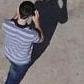
\includegraphics[width=0.5\textwidth]{figures/bb0 (1).jpg}
            \caption{}
            \label{fig:enter-label}
    \end{subfigure}%
    \begin{subfigure}{0.3\textwidth}
            \centering
            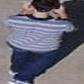
\includegraphics[width=0.5\textwidth]{figures/bb131.jpg}
            \caption{}
            \label{fig:enter-label}
    \end{subfigure}%
    \begin{subfigure}{0.3\textwidth}
            \centering
            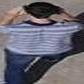
\includegraphics[width=0.5\textwidth]{figures/bb1513.jpg}
            \caption{}
            \label{fig:enter-label}
    \end{subfigure}%
    \begin{subfigure}{0.3\textwidth}
            \centering
            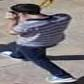
\includegraphics[width=0.5\textwidth]{figures/bb6928.jpg}
            \caption{}
            \label{fig:enter-label}
    \end{subfigure}
\end{subfigure}

\begin{subfigure}{0.7\textwidth}
    \begin{subfigure}{0.3\textwidth}
            \centering
            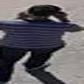
\includegraphics[width=0.5\textwidth]{figures/bb12113.jpg}
            \caption{}
            \label{fig:enter-label}
    \end{subfigure}%
    \begin{subfigure}{0.3\textwidth}
            \centering
            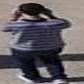
\includegraphics[width=0.5\textwidth]{figures/bb22585.jpg}
            \caption{}
            \label{fig:enter-label}
    \end{subfigure}%
    \begin{subfigure}{0.3\textwidth}
            \centering
            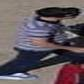
\includegraphics[width=0.5\textwidth]{figures/bb33687.jpg}
            \caption{}
            \label{fig:enter-label}
    \end{subfigure}%
    \begin{subfigure}{0.3\textwidth}
            \centering
            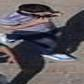
\includegraphics[width=0.5\textwidth]{figures/bb45599.jpg}
            \caption{}
            \label{fig:enter-label}
    \end{subfigure}
\end{subfigure}
\caption{(a)Selected Query Image in First Frame Frame,(b)10th Frame Object Proposal,(c)100th Frame Object Proposal,(d)500th Frame Object Proposal,(e)1000th Frame Object Proposal,(f)2000th Frame Object Proposal,(g)3000th Frame Object Proposal,(h)4000th Frame Object Proposal}
\label{fig:Second Case}
\end{figure}

\begin{figure}[H]
    \centering
    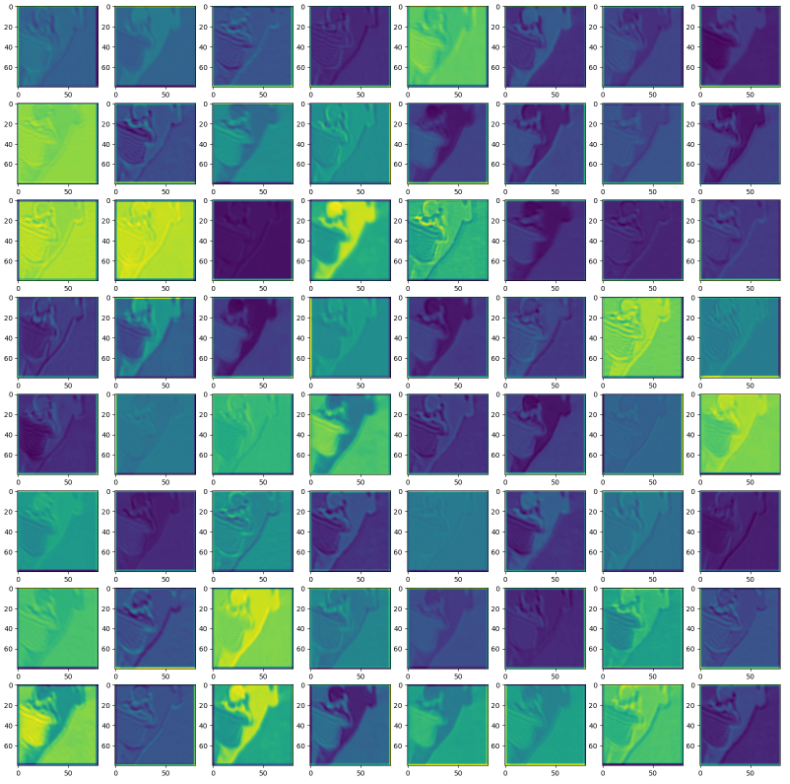
\includegraphics[width=0.5\textwidth]{figures/Layer_4_First_Image.png}
    \caption{Feature Map of Selected Query Image in First Frame Frame}
    \label{fig:enter-label}
\end{figure}
\begin{figure}[H]
    \centering
    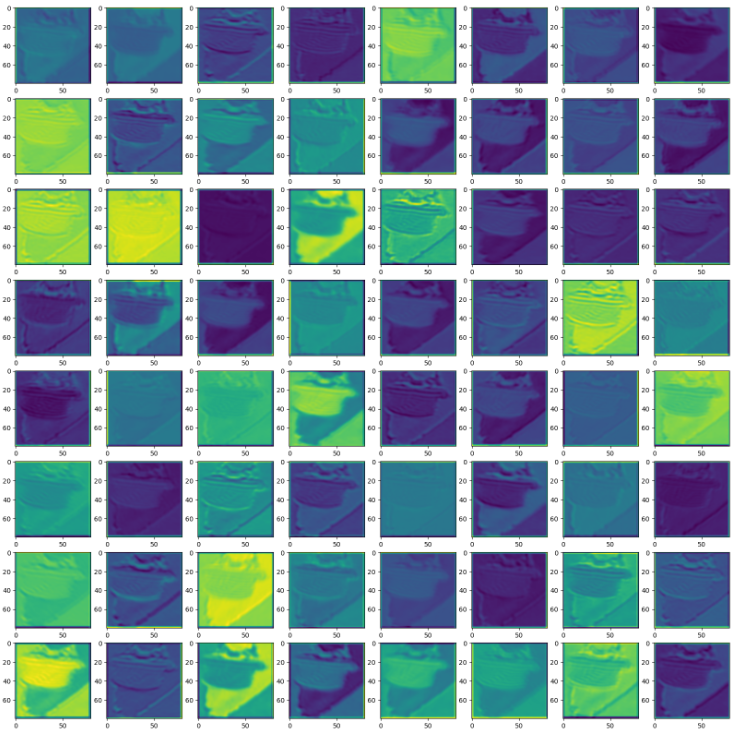
\includegraphics[width=0.5\textwidth]{figures/Layer_4_BB131.png}
    \caption{Feature Map of 10th Frame Object Proposal}
    \label{fig:enter-label}
\end{figure}
\begin{figure}[H]
    \centering
    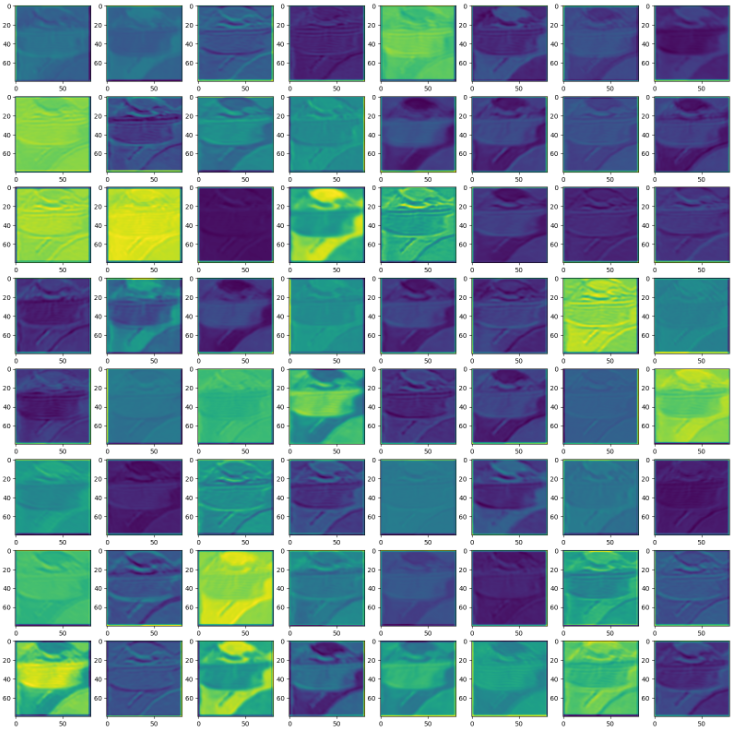
\includegraphics[width=0.5\textwidth]{figures/Layer_4_BB1513.png}
    \caption{Feature Map of 100th Frame Object Proposal}
    \label{fig:enter-label}
\end{figure}
\begin{figure}[H]
    \centering
    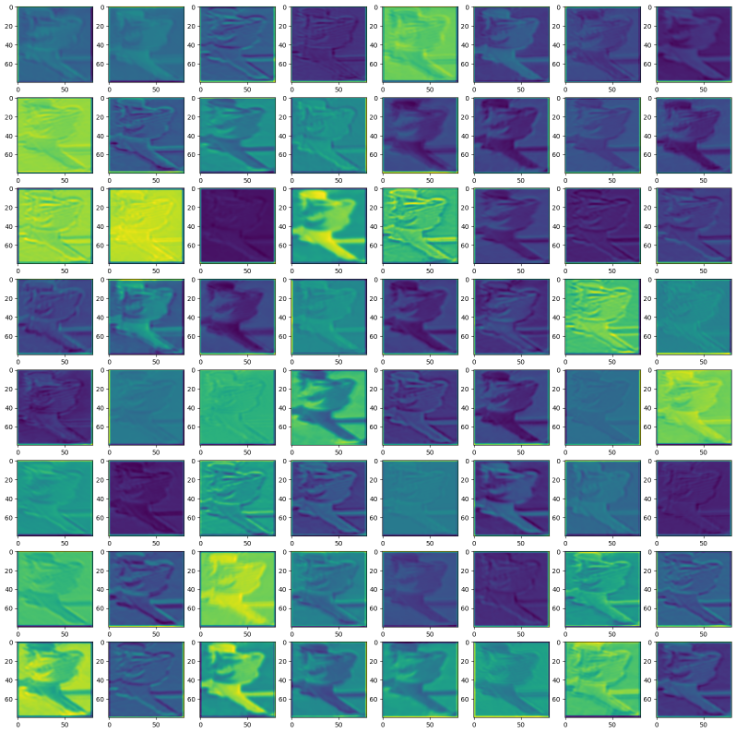
\includegraphics[width=0.5\textwidth]{figures/Layer_4_BB6928.png}
    \caption{Feature Map of 500th Frame Object Proposal}
    \label{fig:enter-label}
\end{figure}
\begin{figure}[H]
    \centering
    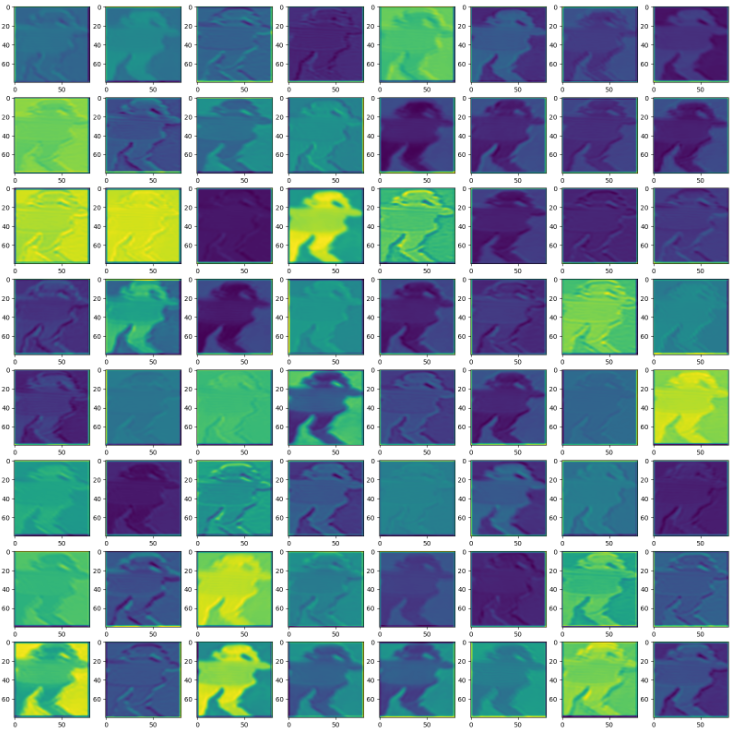
\includegraphics[width=0.5\textwidth]{figures/Layer_4_BB12113.png}
    \caption{)Feature Map of 1000th Frame Object Proposal}
    \label{fig:enter-label}
\end{figure}
\begin{figure}[H]
    \centering
    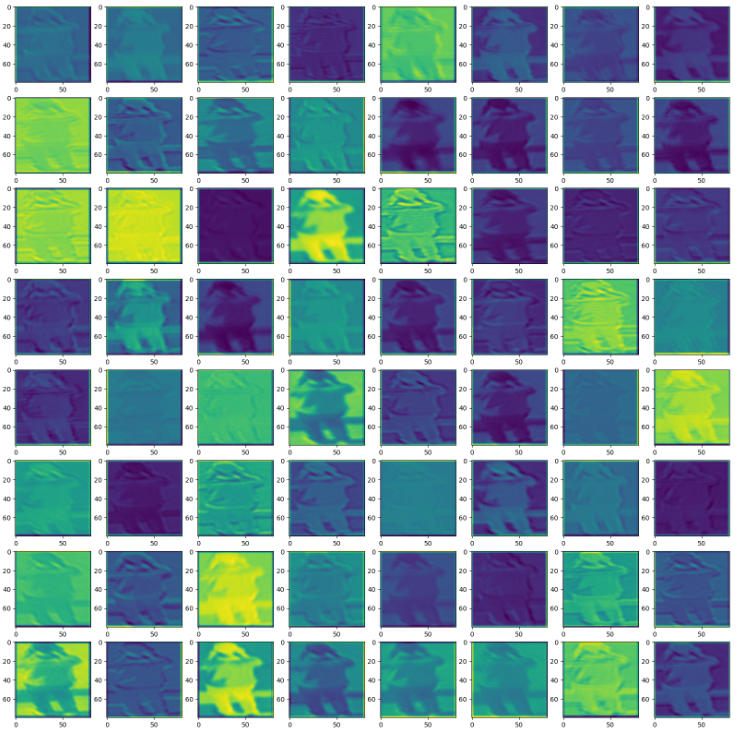
\includegraphics[width=0.5\textwidth]{figures/Layer_4_BB22585.png}
    \caption{Feature Map of 2000th Frame Object Proposal}
    \label{fig:enter-label}
\end{figure}
\begin{figure}[H]
    \centering
    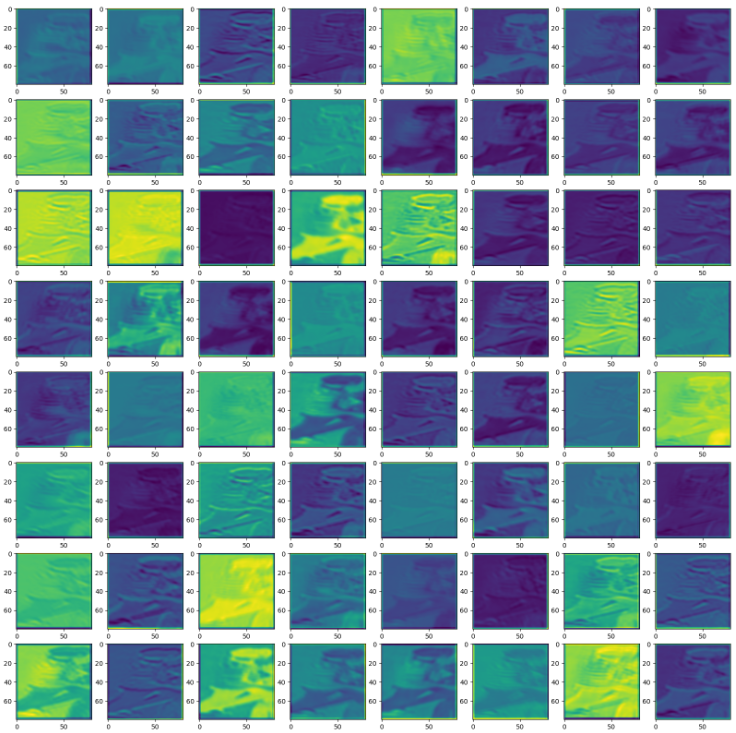
\includegraphics[width=0.5\textwidth]{figures/Layer_4_BB33687.png}
    \caption{Feature Map of 3000th Frame Object Proposal}
    \label{fig:enter-label}
\end{figure}
\begin{figure}[H]
    \centering
    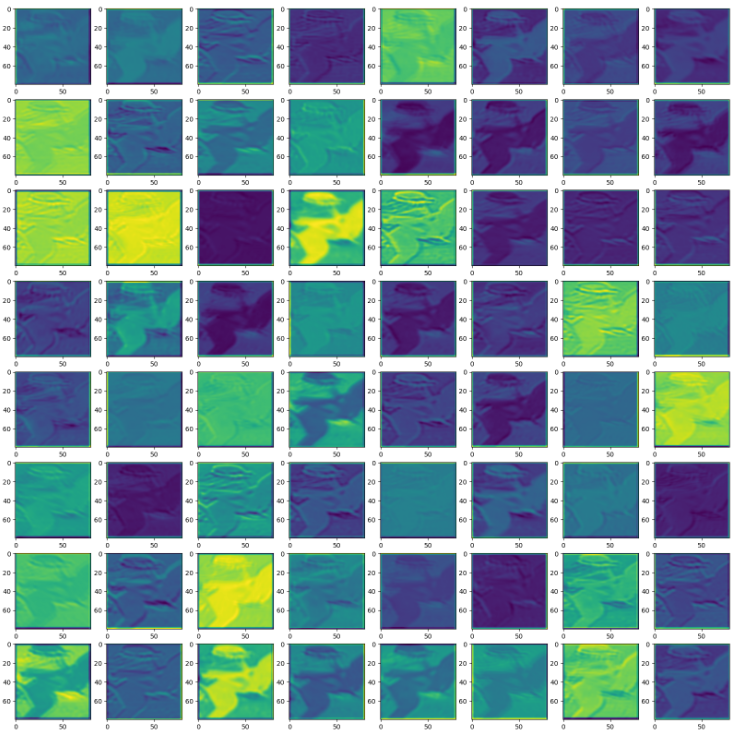
\includegraphics[width=0.5\textwidth]{figures/Layer_4_BB45599.png}
    \caption{Feature Map of 4000th Frame Object Proposal}
    \label{fig:enter-label}
\end{figure}

In the second test case, first proposal which belongs to target object’s class in the first frame was selected as first query image. But this time, query image was updated each and every five frames by selecting object proposal that has same class label with target object. Thus query image nearly indistinguishable with target object proposals in the upcoming frames. This situation can be seen in the \textbf{figure \ref{fig:Second Case}} below. Therefore probability of network to detect proposals as same class with query image significantly increases.

\begin{figure}[H]
\begin{subfigure}{0.7\textwidth}
    \begin{subfigure}{0.3\textwidth}
            \centering
            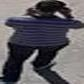
\includegraphics[width=0.5\textwidth]{figures/bb999.jpg}
            \caption{}
            \label{fig:enter-label}
    \end{subfigure}%
    \begin{subfigure}{0.3\textwidth}
            \centering
            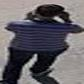
\includegraphics[width=0.5\textwidth]{figures/bb12125.jpg}
            \caption{}
            \label{fig:enter-label}
    \end{subfigure}%
    \begin{subfigure}{0.3\textwidth}
            \centering
            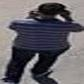
\includegraphics[width=0.5\textwidth]{figures/bb12133.jpg}
            \caption{}
            \label{fig:enter-label}
    \end{subfigure}%
    \begin{subfigure}{0.3\textwidth}
            \centering
            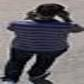
\includegraphics[width=0.5\textwidth]{figures/bb12140.jpg}
            \caption{}
            \label{fig:enter-label}
    \end{subfigure}%
    \begin{subfigure}{0.3\textwidth}
            \centering
            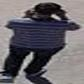
\includegraphics[width=0.5\textwidth]{figures/bb12152.jpg}
            \caption{}
            \label{fig:enter-label}
    \end{subfigure}
\end{subfigure}
\caption{(a)Selected Query Image in 1000th Frame,(b)1001th Frame Object Proposal,(c)1002th Frame Object Proposal,(d)1003th Frame Object Proposal,(e)1004th Frame Object Proposal}
\label{fig:Second Case}
\end{figure}



In order to test these assumptions decision criteria was needed to be selected to classify unlabeled proposals. Therefore \textbf{IoU(Intersection Over Union)} and relation scores of query images and proposals were used to decide if a proposal has same class label with query image.In the \textbf{figure \ref{fig:IoUvsProposalAmount}} total amounts of proposals were assigned to corresponding IoU score intervals. The proposals which have 0.1 or greater IoU score and the highest relation score between support images were determined as true positives.
%Bu kısımda kafam karıştı. Tam nasıl anlatacağımı sor. Proposallar farklı boyutlara sahip olduğu için iou 0.1'e kadar düşüyor. Skorlardan nasıl bir çıkarım yapmam gerekiyor? Zaten relation scores arasından en büyüğünü alıyorum. Bu da minimum 2.6 falan. Asıl sorum buradan tam nasıl bir çıkarım yapmam gerekiyor? 


\begin{figure}[H]
    \centering
    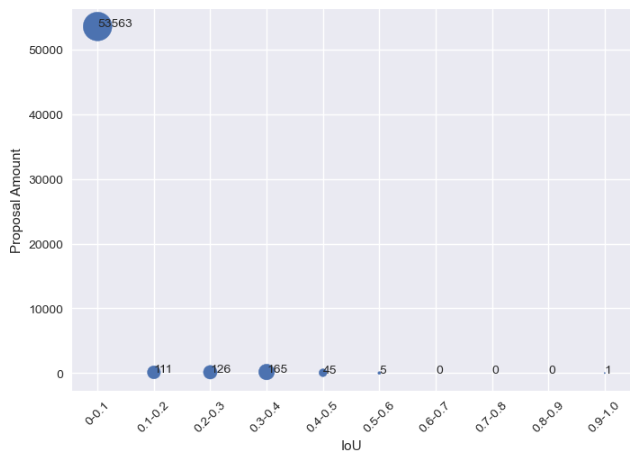
\includegraphics[width=0.8\textwidth]{figures/IoUvsProposalAmount.png}
    \caption{Distribution of proposals according to IoU scores.}
    
    \label{fig:IoUvsProposalAmount}
\end{figure}

\begin{figure}[H]
    \centering
    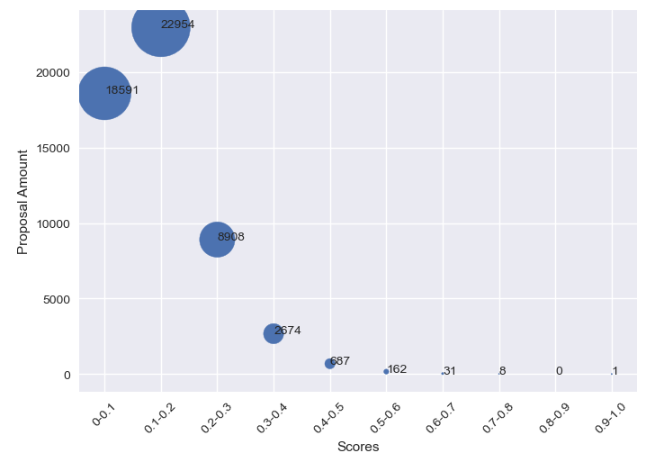
\includegraphics[width=0.8\textwidth]{figures/ScoresvsProposalAmount.png}
    \caption{Distribution of proposals according to relation scores.}
    
    \label{fig:RelationScoresvsProposalAmount}
\end{figure}

\begin{figure}[H]
    \centering
    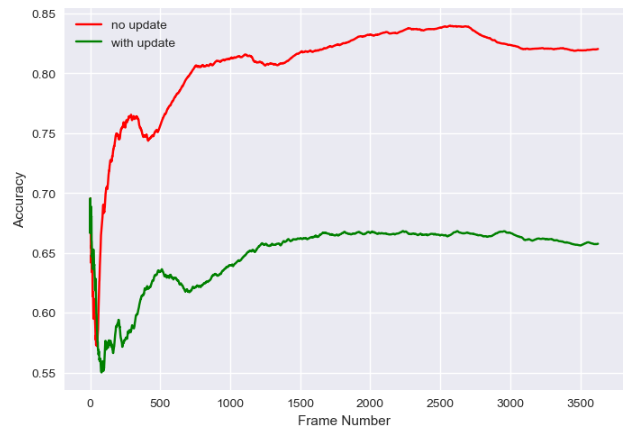
\includegraphics[width=0.9\textwidth]{figures/Final_ACC_Comparison.png}
    \caption{Accuracy comparison between first test case and second test case.}
    \label{fig:ACC Comparison}
\end{figure}

\textbf{Accuracy} is defined as follows,
\[
\frac{True\hspace{0.05in}Positives + True\hspace{0.05in}Negatives}{True\hspace{0.05in}Positives + True\hspace{0.05in}Negatives + False\hspace{0.05in}Positives + False\hspace{0.05in}Negatives}
\]
%Hocam siz accuracy formülünü değiştir dediniz ama internette gördüğüm bir bu var. Ancak deniyor ki classlara ait örnek sayısının dengeli olmadığı deneylerde accuracy yanlış sonuçlar çıkarabiliyor o yüzden recall ve precision kısmına baktım. Onlar da doğru gözüküyor. Kodu da kontrol ettim ara ara resimlere bakıp her yönden check ettim. Bu grafiklerle ilgili yorumum şu: Network resimleri ayırt etmekte iyi olduğu için true negatif sayısı çok artıyor dolayısıyla accuracy de artıyor  gibi görünüyor ancak bizim asıl amacımız daha az sayıdaki true pozitifleri bulmak olduğu için recall ve precision kısmı daha önemli. Zaten ikinci test durumu da az sayıdaki doğru örneği bulmakta daha iyi olduğunu göstermiş oluyor. 
It is a metric which gives the ratio between data which has been predicted correctly and the total data which was given to the model as an input. As can be seen in the \textbf{figure \ref{fig:Second Case}}, as the frame number increases, selected query images have more similarity with the proposals which have same class label since they are updated frequently. RN's feature extractor's output feature maps also show similar patterns for these images as can be seen in the figure  feature map kıyaslaması gelecek.Whereas first test case features are lack of similarity. Therefore second test case's accuracy score was expected to be higher. Also query image which was selected in the first test case has a lower probability to found out to be has same class label with proposals which are shown in the \textbf{figure \ref{fig:Second Case}} by RN because of the difference between target object's angle and lack of proper lighting.Effects of these attributes are quietly noticeable in the feature maps which are shown in the \textbf{figure \ref{fig:Feature Map Comparison}}. But test resulted that accuracy scores of the first test case are higher than the second case as can be seen in the \textbf{figure \ref{fig:Second Case}}. Although accuracy has an important role for final decision it's not sufficient by itself. Therefore other performance metrics such as \textbf{Recall(True Positive Rate)} and \textbf{Precision} are needed to be examined before final decision. 

Recall is a metric which can be described as the ration between proposals which were detected as positive and the amount of proposals which were needed to be detected as positive.Since main focus of this study is improving object tracking capabilities of a network.

\textbf{Recall} is defined as follows,
\[
\frac{True\hspace{0.05in}Positives}{True\hspace{0.05in}Positives + False\hspace{0.05in}Negatives}
\]

\textbf{Figure \ref{fig:Recall Comparison}} shows that in the second test case, RN was clearly better at detecting the proposal as positive which were needed to be detected as positive.In the first test case, network fails to detect positive proposals after certain frame number.   

\begin{figure}[H]
    \centering
    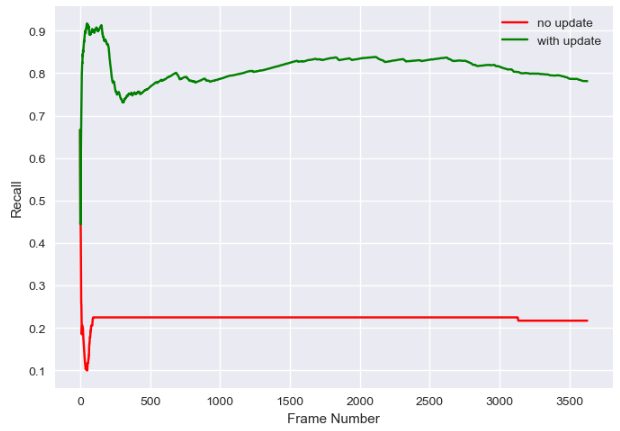
\includegraphics[width=0.9\textwidth]{figures/Final_Recall_Comparison.png}
    \caption{Recall comparison between first test case and second test case.}
    \label{fig:Recall Comparison}
\end{figure}


Precision is a metric which can be described as actual positives among the proposals which were detected as positive.

\textbf{Precision} is defined as follows,
\[
\frac{True\hspace{0.05in}Positives}{True\hspace{0.05in}Positives + False\hspace{0.05in}Positives}
\]



\begin{figure}[H]
    \centering
    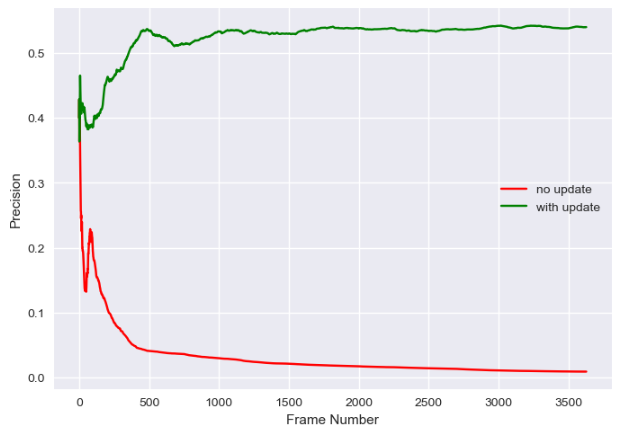
\includegraphics[width=0.9\textwidth]{figures/Final_Precision_Comparison.png}
    \caption{Precision comparison between first test case and second test case.}
    \label{fig:Precision Comparison}
\end{figure}

Recall, is a metric that shows the ratio between the samples which was estimated as positive and how much of the samples were needed to be estimated as positive. Since main focus of this study is improving object tracking capabilities of a network and object tracking is generally done by detecting as much positive samples which share same class label with target object as possible. Therefore in the second test case, relation network has a better performance at detecting similar images because of the update rule. To better understand this situation confusion matrixes in the \textbf{figure \ref{fig:Confusion Matrix Comparison}} should be analyzed. 


\begin{figure}[H]
\centering
\begin{subfigure}{0.9\textwidth}
    \centering
    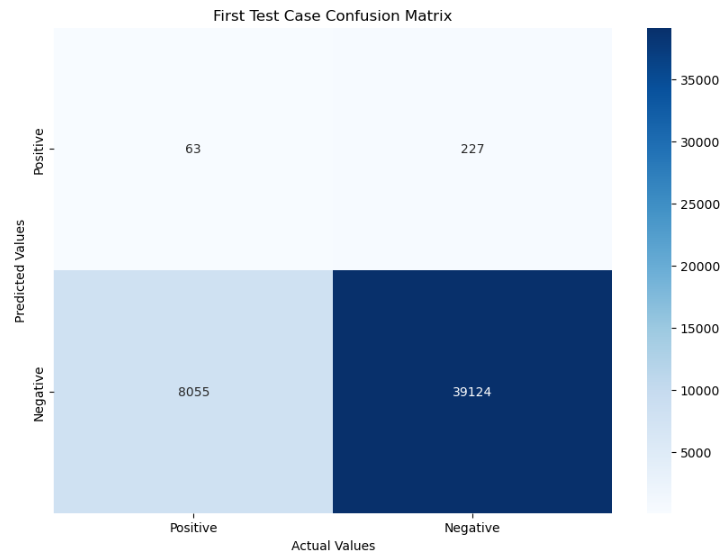
\includegraphics[width=0.9\textwidth]{figures/FT_Final_ConfusionMatrix.png}
    \caption{Caption}
    \label{fig:Second Case Query}
\end{subfigure}
\begin{subfigure}{0.9\textwidth}
    \centering
    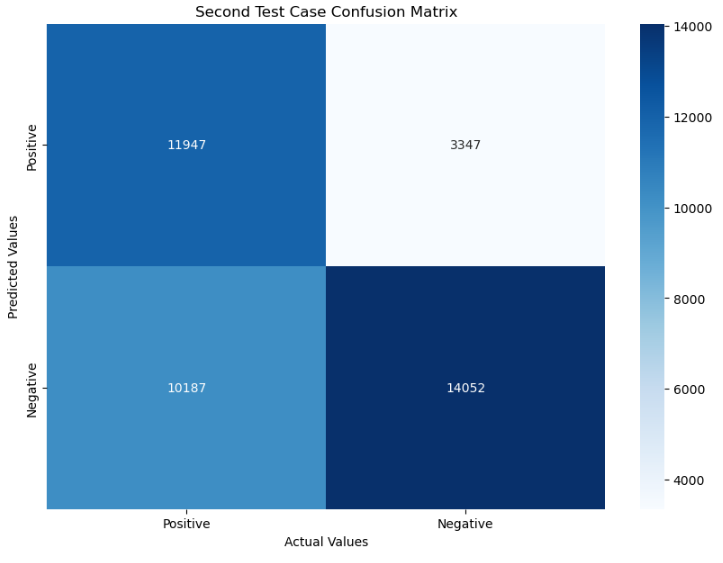
\includegraphics[width=0.9\textwidth]{figures/SC_Final_ConfusionMatrix.png}
    \caption{Caption}
    \label{fig:enter-label}
\end{subfigure}
\caption{Comparison of confusion matrixes of first test case and second test case}
\label{fig:Confusion Matrix Comparison}
\end{figure}





\section{Conclusions}
\lipsum[100]  

%\bibliographystyle{unsrt}
%\bibliography{references} % The filename of the bibliography


\end{document}


